\section{Results}

\subsection{Evaluator dependence and the held-out evaluation boundary}

The retrospective 12-checkpoint screen showed that the fixed fusion candidates
varied in magnitude and, in some cases, sign across detectors and domains
(Fig.~\ref{fig:core}a). For example, CDF was positive on LLVIP and near zero on
the M3FD and DroneVehicle evaluators, whereas SPGFusion was strongly negative
on several LLVIP checkpoints and positive on DroneVehicle. The preferred input
therefore changed even when the fused images were held fixed. This retrospective
matrix uses the maximum-cardinality study protocol and is descriptive. The
held-out LLVIP and VEDAI contrasts use the standard confidence-ordered matching
described in Methods. Complete checkpoint values and intervals are reported in the
Supplementary Material.
One percentage point corresponds to a change of 0.01 in AP50.

\subsection{Held-out evidence isolates an AP50 switching effect}

Across the six final LLVIP checkpoints, the primary visible contrast was
\(+0.00012\) \([-0.00484,+0.00670]\). CS-ECF was also below Always CDF by
\(0.00446\), with an interval crossing zero. Against the no-shield
selector, the equal-sequence AP50 gain was \(+0.00894\)
\([+0.00096,+0.02155]\), and all six checkpoints were positive. The observed
worst-checkpoint loss fell from 0.03270 to 0.00451
(Table~\ref{tab:main-comparison} and Fig.~\ref{fig:core}).
This no-shield comparison was secondary in the local protocol and is treated
as held-out exploratory evidence rather than as the primary endpoint.
The direct no-shield-minus-visible contrast was \(-0.00881\)
\([-0.02593,+0.00256]\). Thus part of the shield's advantage over no shield is
recovery from a selector that was worse than visible, not a gain over visible.

The switch-budget control sharpened the attribution. A random policy matched
to the exact per-checkpoint switch count and candidate multiset had a median
contrast of \(-0.01380\) relative to visible. CS-ECF exceeded that median by
\(+0.01392\) \([+0.00964,+0.02023]\). Its observed worst-checkpoint gain
\(-0.00451\) was also smaller in magnitude than the matched-random median
\(-0.03117\). This supports an image-level selection effect beyond the
reduction in switching frequency.

The VEDAI external-domain test showed the same boundary. CS-ECF remained below
visible input by 0.0136, with an interval below zero, and below Always CDF by
0.0242. It separated from no-shield selection by \(+0.0410\)
\([+0.0097,+0.0782]\), with both training runs positive. Results from the two
new DroneVehicle runs were heterogeneous and are reported as a sensitivity
analysis. When evaluated with AP50--95, CS-ECF minus no shield was \(-0.00009\)
\([-0.00583,+0.00800]\) over LLVIP, with only two positive checkpoints. The
AP50 benefit therefore did not extend to stricter localization. For the two
new DroneVehicle runs, the CS-ECF-minus-visible contrasts were \(-0.00038\)
\([-0.00640,+0.00615]\) and \(+0.00207\) \([+0.00122,+0.00260]\) under
confidence-ordered matching, with an equal-run mean of \(+0.00085\). Their
opposite signs are retained rather than summarised as a uniform domain effect.

\begin{table}[t]
\centering
\small
\setlength{\tabcolsep}{3pt}
\caption{Held-out and external-domain comparisons under standard
confidence-ordered matching. Values are AP50 differences relative to the named
comparator. LLVIP intervals are conditional sequence-by-run summaries; VEDAI
intervals resample ten blocks and two training runs. DroneVehicle intervals
resample three fixed blocks and two independent runs. The VEDAI block
estimand averages the classes present in each block, not a fixed five-class
set. DroneVehicle is reported by independent run and as an equal-run summary.
Full checkpoint- and block-level results are provided in the Supplementary
Material.}
\label{tab:main-comparison}
\begin{tabular}{@{}lcccc@{}}
\toprule
Scope & Visible & Always CDF & No shield & Positive \\
\midrule
LLVIP, six final & \(+0.00012\) & \(-0.00446\) & \(+0.00894\) & 6/6 vs NS \\
VEDAI, equal run & \(-0.0136\) & \(-0.0242\) & \(+0.0410\) & 2/2 vs NS \\
DroneVehicle, run 1 & \(-0.00038\) & \(+0.01198\) & \(+0.00760\) &
1/1 vs NS \\
DroneVehicle, run 2 & \(+0.00207\) & \(+0.00555\) & \(+0.00500\) &
1/1 vs NS \\
DroneVehicle, equal run & \(+0.00085\) & \(+0.00877\) & \(+0.00630\) &
2/2 vs NS \\
\bottomrule
\end{tabular}
\end{table}

The fixed CDF comparison reinforced this boundary. On the LLVIP test, Always CDF
was above CS-ECF by 0.00446; on VEDAI the gap was 0.0242 and CS-ECF also
remained below visible input (Fig.~\ref{fig:core}). The results therefore do
not support replacing a stable fixed fusion input with the shield. They support
only the narrower use of the shield when an unconstrained per-image selector
can produce a large AP50 regression.

\begin{figure}[H]
\centering
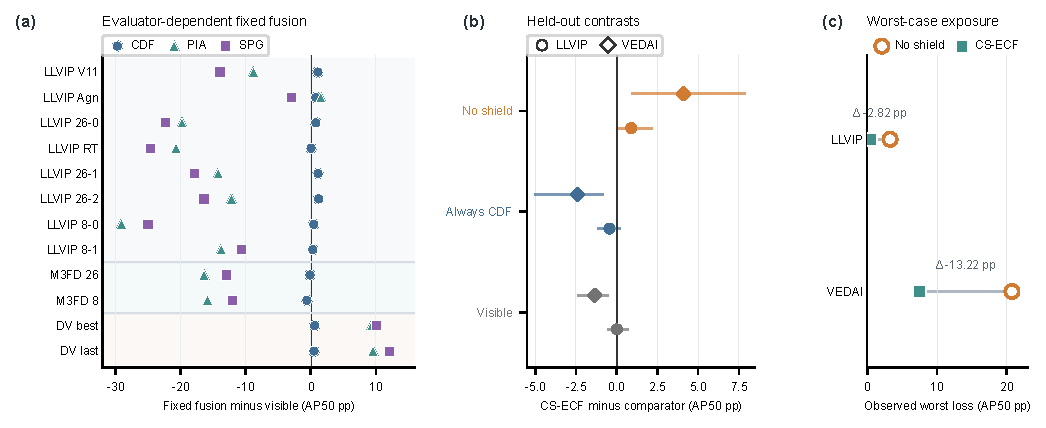
\includegraphics[width=\linewidth]{Figure3_core_evidence.pdf}
\caption{\textbf{Core evidence for detector-conditioned arbitration.}
(\textbf{a}), Fixed CDF, PIAFusion, and SPGFusion differences from visible
across 12 retrospective checkpoints directly show evaluator-dependent sign
changes. Abbreviations are expanded in the source data. (\textbf{b}), Held-out
LLVIP and VEDAI comparisons with standard confidence-ordered matching.
(\textbf{c}), Observed worst-loss reduction of CS-ECF relative to no shield.
Panel (a) is descriptive and uses the study's maximum-cardinality protocol;
panels (b,c) use standard matching and conditional resampling intervals.
Source data are provided in \texttt{Figure3\_source.csv}.}
\label{fig:core}
\end{figure}

\subsection{Budgeted candidate-library selection}

At the frozen \(K=5\) and margin \(1.5\), the development-feasible minimum
subset was visible plus PIAFusion. Its mean development gain was
\(+0.00206\), its worst evaluator gain was \(+0.00039\), and all four
evaluator cells were positive. The four-candidate policy had a lower
development mean of \(+0.00085\), one negative evaluator, and a worst gain of
\(-0.00007\). The selected subset therefore eliminated SPGFusion and CDF
without losing validation performance.

On the standard-matched LLVIP holdout, the selected subset gained
\(+0.00337\) \([-0.00016,+0.01267]\) AP50 over visible input, with five of six
positive checkpoints and a worst-checkpoint loss of \(0.00043\). Relative to
no-shield selection, the gain was \(+0.01218\) \([+0.00136,+0.02915]\), with all
six checkpoints positive. Relative to the full four-candidate CS-ECF policy,
the observed mean difference was \(+0.00325\)
\([-0.00026,+0.01051]\). Its AP50--95 contrast versus visible was
\(+0.00221\) \([-0.00006,+0.00788]\), with six of six positive checkpoints.
These intervals remain conditional on the observed scene, checkpoint, and
block hierarchy.

Because that evaluation followed subset selection, we recorded a new temporal
protocol before scoring LLVIP sequences 080, 090, and 100. The fixed sample
contains 300 non-empty frames per sequence. The policy and margin were
unchanged. It gained \(+0.01560\) \([+0.00249,+0.02874]\) AP50 over visible,
with positive equal-sequence gains of \(+0.02543\), \(+0.01924\), and
\(+0.00213\), and positive gains on all six checkpoints. The worst checkpoint
gained \(+0.00784\). The AP50--95 contrast was \(+0.00946\)
\([+0.00113,+0.01769]\).

A post hoc leave-one-sequence-out sensitivity check retained a gain between
\(+0.01068\) and \(+0.02233\) after omitting any one sequence, with all six
checkpoints positive in each analysis.

The gate, rather than PIAFusion itself, produced this result. Always using
PIAFusion had an equal-sequence AP50 change of \(-0.01237\)
\([-0.15111,+0.07787]\). Its sequence values were \(+0.05415\), \(+0.06766\),
and \(-0.15891\). The frozen rule switched \(5.22\%\) of image-checkpoint
cases, tied on \(95.20\%\), won on \(4.22\%\), and lost on \(0.57\%\). The gain
is therefore concentrated in the images that pass the confidence margin.
This temporal confirmation does not remove the negative VEDAI and
DroneVehicle results.

The external boundary was not removed. The same frozen two-candidate policy
was \(-0.00329\) \([-0.00884,+0.00011]\) AP50 relative to visible on VEDAI and
\(-0.00124\) \([-0.00578,+0.00280]\) on the two independent DroneVehicle runs.
It remained better than no-shield selection on average in both domains
(\(+0.05131\) and \(+0.00421\)), but not relative to visible. Across the three
external evaluators the visible-relative difference was \(+0.01844\)
\([+0.00187,+0.03871]\); this is descriptive because those evaluators differ
in training modality and the interval spans only seven scenes. The selected
subset thus reduces the cost of a validated policy. It is not a universal
accuracy gain, and a failed target-domain validation returns visible input.

\begin{figure}[H]
\centering
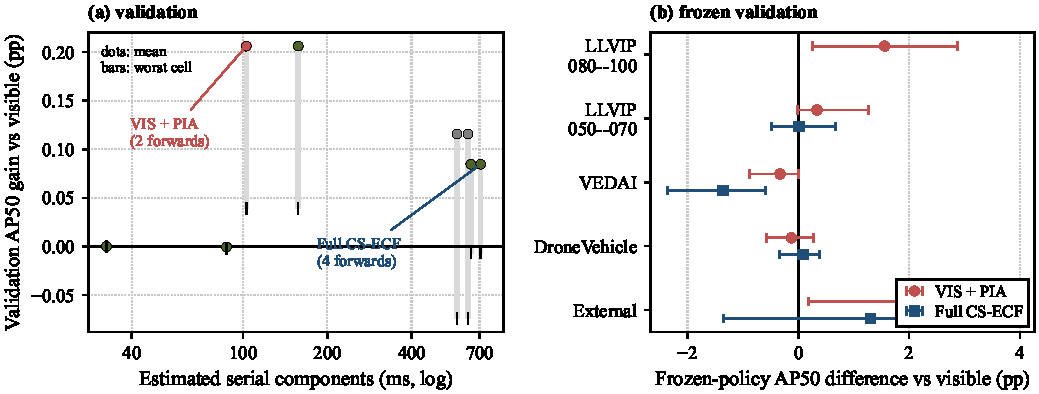
\includegraphics[width=\linewidth]{FigureBudgetedSelection.pdf}
\caption{\textbf{Budgeted candidate-library selection and transfer boundary.}
(\textbf{a}), Development evaluator mean and worst-cell AP50 gain at the
fixed \(K=5\), margin \(1.5\) policy. Each point is a candidate subset; the
horizontal position is the estimated serial component cost. The filled red
point is the selected visible plus PIAFusion subset. (\textbf{b}), Frozen
policy evaluated against visible input. The first row is the later LLVIP
temporal confirmation; subsequent rows are earlier LLVIP 050--070, VEDAI,
independent DroneVehicle, and external-evaluator tests. Only the selected
policy was rescored in the new temporal holdout. Symbols are equal-sequence or
equal-run means and intervals are conditional resampling summaries. External
domains remain exploratory. Source data are provided in
\texttt{FigureBudgetedSelection\_source.csv}.}
\label{fig:budgeted}
\end{figure}

\subsection{System-level joint-detection reference}

We also trained the recent YOLOv11-RGBT early-fusion detector on the same
1,600/400/200 M3FD split and 40-epoch budget
(Table~\ref{tab:joint-baseline}). This system accepts a four-channel
visible--infrared image and optimizes fusion and detection together. Because
both the representation and detector change, we use its result only to
document one reproducible end-to-end implementation. The within-checkpoint
comparisons remain the evidence for the selector. The visible baselines use a
different optimization schedule, the joint model is run once, and several rare
classes are poorly represented in its score. We therefore make no performance
ranking from Table~\ref{tab:joint-baseline}.

\begin{table}[t]
\centering
\small
\caption{System-level M3FD comparison. The visible-trained rows use the same
held-out test groups and the study AP protocol. YOLOv11-RGBT jointly trains
four-channel fusion and detection and is not an architecture-matched
comparator. Its single-seed, resize-only pilot is not an estimate of best
attainable performance or evidence of intrinsic framework inferiority. Source
data are provided in
\texttt{TableJointBaseline\_source.csv}.}
\label{tab:joint-baseline}
\begin{tabular}{@{}llc@{}}
\toprule
System & Input setting & AP50 \\
\midrule
YOLO26n & visible-only checkpoint & 0.3717 \\
YOLO26n & CS-ECF on the same checkpoint & 0.3757 \\
YOLOv8n & visible-only checkpoint & 0.3790 \\
YOLOv8n & CS-ECF on the same checkpoint & 0.3972 \\
YOLOv11-RGBT & joint four-channel fusion and detection & 0.0963 \\
\bottomrule
\end{tabular}
\end{table}

The pooled AP50 entries in Table~\ref{tab:joint-baseline} are not the paired
estimand. On the two M3FD held-out frame groups, the equal-group
CS-ECF-minus-visible differences were \(+0.00291\) \([0.00000,+0.00582]\) for
YOLO26n and \(+0.01281\) \([0.00000,+0.02561]\) for YOLOv8n. Both intervals
are conditional on only two frame groups. Each evaluator in that archive
represented one training run. After the policy had been frozen, we trained
seeds 1 and 2 for both families with the same 40-epoch recipe and jointly
rescored all six checkpoints against the four candidates. The CS-ECF gain over
visible input was positive in all 6 of 6 runs. Its pooled mean was \(+0.00852\)
(range \(+0.00179\) to \(+0.01809\)), and its equal-group mean was \(+0.00617\)
(range \(+0.00175\) to \(+0.01278\)). The variation across seeds was
substantial, but every within-run contrast remained positive. The six runs
still represent two model families and only two held-out frame groups. Absolute
AP50 values in this jointly rescored archive are therefore compared only within
run and not with earlier archive values. These results strengthen the observed
within-run direction without creating cross-domain confirmation.
Run-level values and source data are provided in the Supplementary Material.

\subsection{Portability and mechanism boundaries}

The frozen selector also operated on three external detector checkpoints.
Both zero-shot evaluators improved on visible input, but no-shield selection
exceeded CS-ECF on both. The equal-scene CS-ECF-minus-no-shield contrasts were
\(-0.0179\) and \(-0.0098\), with intervals crossing zero. An LLVIP-trained
YOLOv9t reversed the visible-relative contrast, with a change of \(-0.0142\);
CS-ECF exceeded no shield there but still remained below visible. Thus neither
the visible-relative gain nor the shield-versus-no-shield ordering transferred
across all checkpoints (Fig.~\ref{fig:external}).

The matched image-statistic audit did not produce a usable operating point at
the CS-ECF switching budget, so the study does not establish a
confidence-specific mechanism. This limitation is part of the result rather
than a claim to be inferred away. Detailed control, calibration, class, and
thermal analyses are retained in the Supplementary Material.

\begin{figure}[H]
\centering
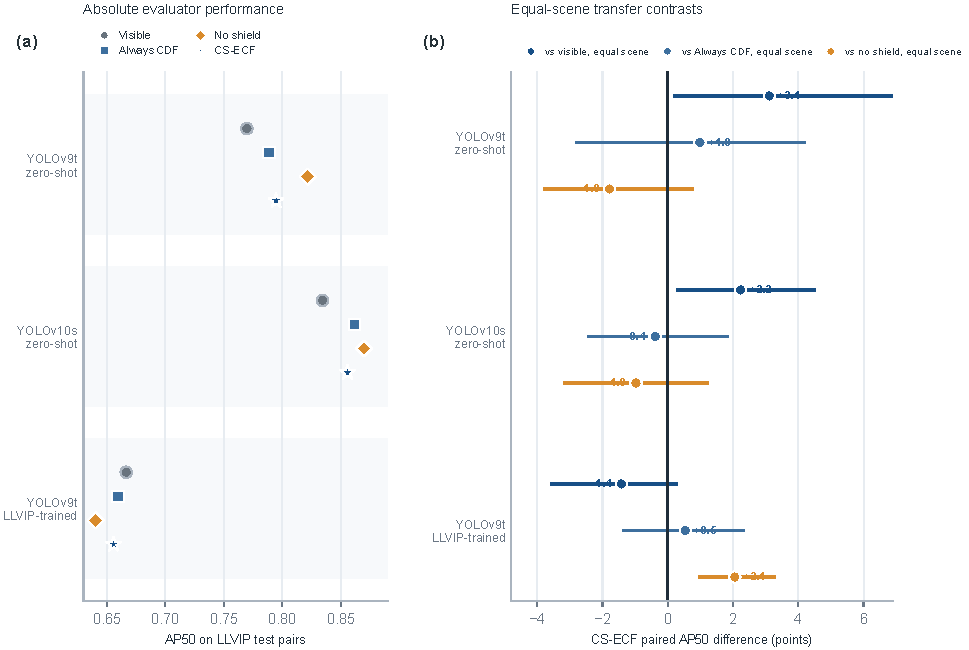
\includegraphics[width=0.90\linewidth]{Figure7_external_evaluators.pdf}
\caption{\textbf{External-evaluator portability stress tests.} Zero-shot
detectors support a visible-relative gain but not CDF superiority, and their
no-shield point estimates exceed CS-ECF. The LLVIP-trained checkpoint reverses
the visible-relative sign while CS-ECF exceeds no shield. Intervals are
descriptive and conditional on seven scene groups. Source data are provided in
\texttt{Figure7\_source.csv}.}
\label{fig:external}
\end{figure}

\subsection{Successful and failed switches}

The selected-case audit illustrates both ends of the decision problem. The
YOLO26n seed-0 checkpoint switched 17 of 1,395 images: 8 improved, 5 degraded,
and 4 were unchanged. For Fig.~\ref{fig:cases}, we selected cases whose matched
true-positive count changed. In the success case, visible input missed the
single annotated pedestrian in sequence frame 070142. SPGFusion produced a true
positive at confidence 0.67 and raised per-image AP50 from 0 to 1. In the failure case,
visible input in frame 070162 matched two of three pedestrians, whereas
SPGFusion retained only one. The examples are illustrative endpoints selected by a fixed rule, not
estimates of the average effect.

\begin{figure}[H]
\centering
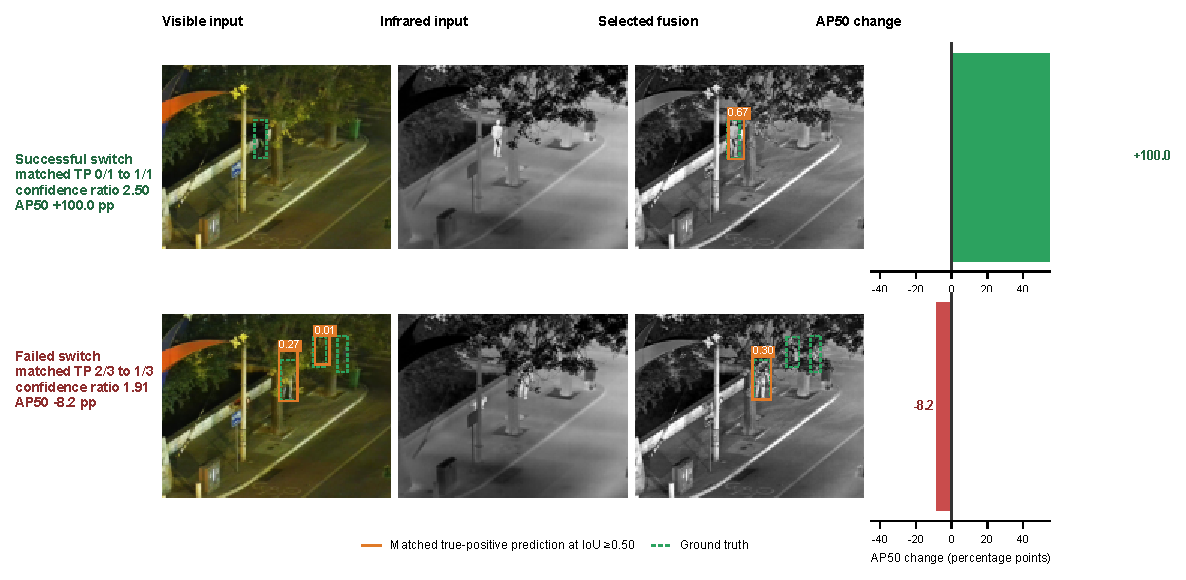
\includegraphics[width=0.96\linewidth]{Figure6_case_studies.pdf}
\caption{\textbf{Successful and failed CS-ECF switches.} The two rows show a
successful and a failed switch from the YOLO26n seed-0 checkpoint over LLVIP
sequences 050, 060, and 070. The examples are frames 070142 and 070162. Cases
were selected by a fixed rule requiring a
change in matched true-positive count that remains visible to a reader. Each
row shows visible input, infrared input, the selected fusion image, and the
paired AP50 change. Solid boxes are matched true-positive predictions at an
IoU of 0.50, annotated with detector confidence; dashed boxes are ground truth.
Ground truth is used only for this explanatory visualization, not for policy
selection. The examples are selected endpoints, not average effects. Source
data are provided in
\texttt{Figure6\_source.csv}.}
\label{fig:cases}
\end{figure}

\subsection{Operational interpretation}

The operational rule is stricter than a minimum-margin rule alone. First, use
visible input when a fused subset fails the development loss bound. Otherwise,
select the smallest feasible candidate subset rather than defaulting to the
full library. Before deployment, reproduce the matched-random comparison and
the candidate-subset check on representative groups for the target checkpoint
and domain. The selected subset should also retain its direction under the
decision-relevant metric and fit the latency and memory budget. A
switching-rate reduction alone, a full-library validation result, or a
development gain in another domain is insufficient. These are validation
gates, not measured operating guarantees (Fig.~\ref{fig:cost}).

\begin{figure}[H]
\centering
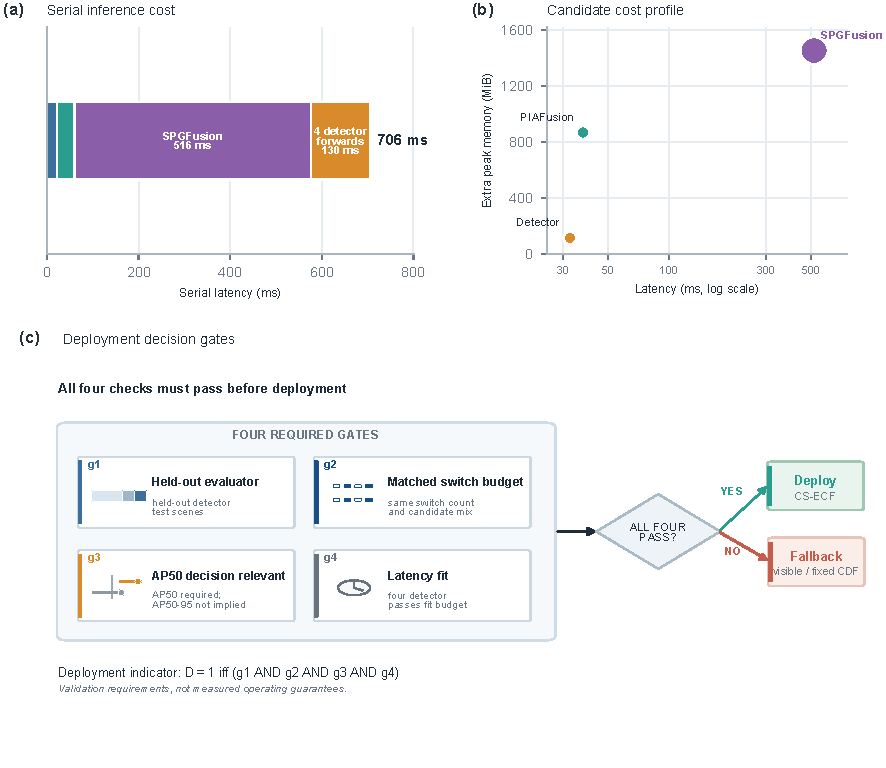
\includegraphics[width=\linewidth]{Figure11_cost_deployment.pdf}
\caption{\textbf{Cost and deployment boundaries.} Component timing,
non-additive peak memory, and four validation gates required before choosing
CS-ECF. A failed gate returns the system to visible input or stable fixed CDF.
The figure does not define a validated deployment threshold or a latency
guarantee. Source data are provided in
\texttt{Figure11\_source.csv}.}
\label{fig:cost}
\end{figure}
